% 3_architecture_robot.tex

\section{Architecture du robot}

\begin{center}
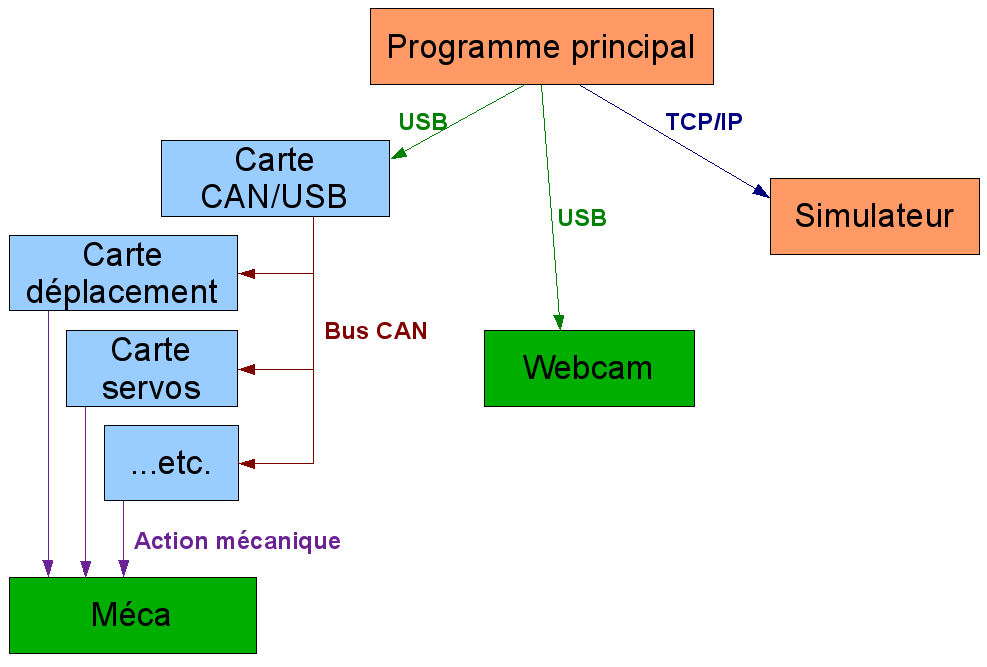
\includegraphics[width=12cm]{images/architecture_1.png}\\
\end{center}
\indent Le robot s'articule en 3 grandes parties : l'informatique, l'électronique et la mécanique. Le programme principal, linké avec les librairies nécessaires (libRobot, libRobot2008, libWebcam...), pilote soit le simulateur par TCP/IP, soit les cartes électroniques, qui elles-mêmes actionnent des servos, des moteurs...etc et pour faire agir le robot. Les cartes électroniques permettent aussi de renvoyer de l'information au programme principal, comme une position sur le terrain, si le robot a une balle à l'intérieur...etc.\\

\begin{center}
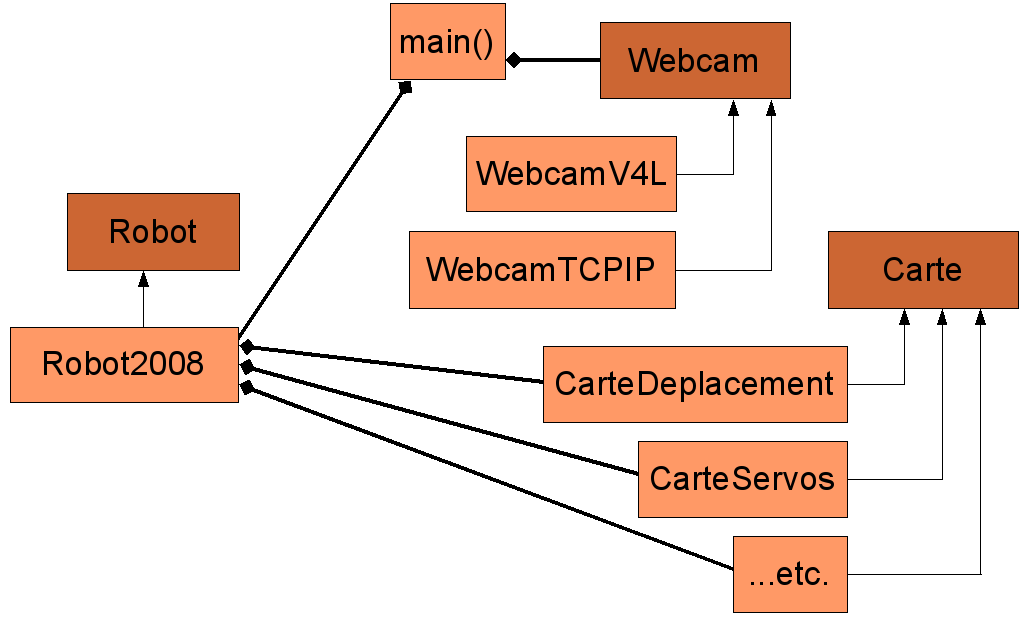
\includegraphics[width=12cm]{images/architecture_2.png}\\
\end{center}
\indent Au niveau de l'organisation des classes, le programme principal, main(), possède 2 instances des classes Robot2008 et WebcamV4L ou WebcamTCPIP. En réalité, le programme principal ne manipule qu'un pointeur Webcam*, la classe Webcam étant une interface permettant de piloter de façon transparente la véritable webcam, via l'API Video4Linux, ou la webcam du simulateur (communication par TCP/IP).\\
\indent La classe Robot2008 dérive de la classe Robot, qui sert de base aux robots de 2007, 2008...etc. Même chose pour les classes représentant les cartes, qui dérivent de la classe générale "Carte". Chaque carte expose une interface permettant de piloter les vraies cartes électroniques. Les instances des cartes appartiennent à Robot2008.\\
En plus clair, cela donne lieu à du code comme ceci :
\begin{lstlisting}
int main(int argc, char* argv[])
{
	Robot2008* robot = NULL;

	// Creation du robot
	if(!creationRobot(&robot, argc, argv))
		return -1;

	robot->initialiser();
	robot->getCarteDeplacement()->avancer(100);
	delete robot;
	return 0;
}
	
\end{lstlisting}

La fonction creationRobot() fait un "\lstinline{new Robot2008()}" (équivalent C++ d'un "\lstinline{malloc(sizeof(Robot2008))}" en C), puis règle certains paramètres pour la carte de déplacement, concernant les vitesses à utiliser. En fonction de ce qui est passé en argument au programme à son lancement, il communiquera soit par TCP/IP (avec le simulateur par exemple), soit par RS232 (avec le vrai robot en général).